\documentclass[compress,aspectratio=169]{beamer}
\usepackage[utf8]{inputenc}
\usepackage{xcolor,soul}
%
\usepackage{amsmath}
\usepackage{amsfonts}
\usepackage{amssymb}
\usepackage[american]{babel}
\usepackage{xspace}
\usepackage{graphicx}
\usepackage{ifthen}
\usepackage{figlatex}
\usepackage{colortbl}
\usepackage[labelformat=empty]{caption}
\renewcommand{\captionfont}{\scriptsize}
\usepackage{listings}
\usepackage{fancyvrb}
\usepackage[absolute,overlay]{textpos}
\usepackage{environ}
\usepackage{dot2texi}
\usepackage{tipa}
\usepackage{pifont,ulsy}
\usepackage{mhchem}
\usepackage{relsize}
\usepackage{array}

\newcolumntype{C}[1]{>{\centering\let\newline\\\arraybackslash\hspace{0pt}}m{#1}}

\usepackage{tabularx}

\newcommand{\myitem}[1]{%
\begin{tabularx}{\linewidth}{@{}l@{}>{\raggedright}X@{}}
\usebeamercolor[fg]{structure}$\bullet$~~ & #1
\end{tabularx}%
}    
\newenvironment{myitemize}{\par}{\par}   

\AtBeginDocument{\renewcommand{\proofname}{{\bf Proof}}}

\makeatletter
\DeclareOptionBeamer{compress}{\beamer@compresstrue}
\ProcessOptionsBeamer

\makeatletter
\let\@@magyar@captionfix\relax
\makeatother

\graphicspath{{figures/}{fig}}

\definecolor{cinnabar}{rgb}{1,0.5,0.5}
\makeatletter
\newcommand\SoulColor{%
  \let\set@color\beamerorig@set@color
  \let\reset@color\beamerorig@reset@color}
\makeatother
\usepackage[most]{tcolorbox}

\newtcolorbox{myblock}[2][]{beamer,title=#2,fonttitle=\sffamily,
  left=1mm,right=1mm,top=1mm,bottom=1mm,arc=2mm,
  colback=black,colupper=white,colframe=yellow,
  coltitle=black,title style={top color=red!70,bottom color=yellow},
  #1}


\RecustomVerbatimCommand{\VerbatimInput}{VerbatimInput}{fontsize=\scriptsize}

\mode<presentation>
{
  \usetheme{Replica}
  \setbeamercovered{transparent}
}

\makeatletter
\let\beamer@writeslidentry@miniframeson=\beamer@writeslidentry
\def\beamer@writeslidentry@miniframesoff{%
  \expandafter\beamer@ifempty\expandafter{\beamer@framestartpage}{}% does not happen normally
  {
    \clearpage\beamer@notesactions%
  }
}
\newcount\beamer@writeslidentry@miniframesoneoversome@counter
\newcount\beamer@writeslidentry@miniframesoneoversome@limit
\beamer@writeslidentry@miniframesoneoversome@counter=1
\newcount\beamer@writeslidentry@miniframesoneoversome@limit
\beamer@writeslidentry@miniframesoneoversome@limit=5
\def\beamer@writeslidentry@miniframesoneoversome{%
  \ifnum\beamer@writeslidentry@miniframesoneoversome@counter=\beamer@writeslidentry@miniframesoneoversome@limit\relax%
    \beamer@writeslidentry@miniframesoneoversome@counter=1\relax%
    \beamer@writeslidentry@miniframeson%
  \else%
    \advance\beamer@writeslidentry@miniframesoneoversome@counter by 1%
    \beamer@writeslidentry@miniframesoff%
  \fi%
}
\newcommand*{\miniframeson}{\let\beamer@writeslidentry=\beamer@writeslidentry@miniframeson}
\newcommand*{\miniframesoff}{\let\beamer@writeslidentry=\beamer@writeslidentry@miniframesoff}
\newcommand*{\miniframesalternate}[1]{%
   \beamer@writeslidentry@miniframesoneoversome@counter=1\relax%
   \beamer@writeslidentry@miniframesoneoversome@limit=#1\relax%
   \let\beamer@writeslidentry=\beamer@writeslidentry@miniframesoneoversome}

% Define the subsectionsonly option for beamer toc
\def\beamer@tocaction@only#1{\only<.(1)>{\usebeamertemplate**{#1}}}
\define@key{beamertoc}{subsectionsonly}[]{\beamer@toc@subsectionstyle{show/only}\beamer@toc@subsubsectionstyle{show/shaded/hide}}
\makeatother

\usepackage{enumerate}
\usepackage{url,xspace}
\usepackage{relsize}
\usepackage[ruled,vlined]{algorithm2e}
\usepackage{subfigure}
\usepackage{graphicx,psfrag}
\usepackage{multirow}
\usepackage{rotating}
\usepackage{pstool}
\usepackage{blkarray}
\usepackage{wasysym}
\usepackage{tikzsymbols}

\def\smiley{\green{\larger[2]\wasyfamily\char44}\xspace}
\def\frownie{\blue{\larger[2]\wasyfamily\char47}\xspace}
\def\quesley{\yyellow{\Neutrey}\xspace}

\usepackage{tipa}
\usepackage{pifont}

\AtBeginDocument{\renewcommand{\proofname}{{\bf Proof}}}
\newcommand{\itemb}{\item[$\bullet$]}
 \newcommand{\un}{1 \hspace{-0.132cm}1}
\newcommand{\ignore}[1]{}

\newcommand<>{\blue}[1]{{\color#2{blue!100!black!100}#1}}
\newcommand<>{\red}[1]{{\color#2{red!80!black}#1}}
\newcommand<>{\green}[1]{{\color#2{green!70!black}#1}}
\newcommand<>{\purple}[1]{{\color#2{blue!50!red}#1}}
\newcommand<>{\yyellow}[1]{{\color#2{yellow!90!black}#1}}

\usepackage{tcolorbox}
\tcbuselibrary{theorems}
\tcbuselibrary{skins}
\tcbuselibrary{fitting}
\newtcolorbox{mythmbox}[2][]{colback=white,fonttitle=\bfseries,enhanced,attach boxed title to top left={xshift=15mm,yshift=-2mm},title=#2,#1}
\newtcbox{mybox}[2][]{fonttitle=\bfseries,enhanced,attach boxed title to top left={xshift=15mm,yshift=-2mm},title=#2,#1}

\usepackage{tikz}
\usetikzlibrary{patterns}
\usetikzlibrary{arrows,shapes}
\usetikzlibrary{shapes.geometric}
\usetikzlibrary{decorations.pathreplacing, calc}

\tcbuselibrary{theorems}
\tcbuselibrary{skins}
\tcbuselibrary{fitting}

\usetikzlibrary{patterns}
\usetikzlibrary{arrows,shapes}
\usetikzlibrary{shapes.geometric}
\usetikzlibrary{decorations.pathreplacing, calc}
\usetikzlibrary{calc}
\usetikzlibrary{arrows,shapes}
\usetikzlibrary{patterns,snakes}
\usetikzlibrary{babel}
\usetikzlibrary{scopes,intersections}
\usetikzlibrary{decorations.pathreplacing}

\usetikzlibrary{patterns,arrows,arrows.meta,shapes,decorations.markings,tikzmark,matrix,fit,positioning,decorations.pathreplacing,calc}
\tikzstyle{vecArrow} = [thick, decoration={markings,mark=at position
   1 with {\arrow[semithick]{open triangle 60}}},
   double distance=1.4pt, shorten >= 5.5pt,
   preaction = {decorate},
   postaction = {draw,line width=1.4pt, white,shorten >= 4.5pt}]
\tikzstyle{innerWhite} = [semithick, white,line width=1.4pt, shorten >= 4.5pt]


\pgfdeclarelayer{background}
\pgfdeclarelayer{foreground}
\pgfsetlayers{background,main,foreground}

\usepackage{pgfplots}

\newcommand*{\boxcolor}{red}
\makeatletter
\renewcommand{\boxed}[1]{\textcolor{\boxcolor}{%
\tikz[baseline={([yshift=-1ex]current bounding box.center)}] \node [rectangle, minimum width=1ex,rounded corners,draw] {\normalcolor\m@th$\displaystyle#1$};}}
\makeatother

\makeatletter
\newsavebox{\measure@tikzpicture}
\NewEnviron{scaletikzpicturetowidth}[1]{%
  \def\tikz@width{#1}%
  \def\tikzscale{1}\begin{lrbox}{\measure@tikzpicture}%
  \BODY
  \end{lrbox}%
  \pgfmathparse{#1/\wd\measure@tikzpicture}%
  \edef\tikzscale{\pgfmathresult}%
  \BODY
}
\makeatother

\usepackage{tikz-timing}
\usetikztiminglibrary{beamer}
\usepackage{sidecap}
\usepackage{tikz}
\usetikzlibrary{calc}
\usetikzlibrary{arrows,shapes}
\usetikzlibrary{patterns,snakes}
\usetikzlibrary{babel}
\usetikzlibrary{scopes,intersections}
\usetikzlibrary{decorations.pathreplacing}

\pgfdeclarelayer{background}
\pgfdeclarelayer{foreground}
\pgfsetlayers{background,main,foreground}



%Macros for prediction drawings.
\newcommand{\fault}[1]{
\draw[->, color=red] ($(#1)+(0.2,1)$) -- ($(#1)+(0.1,0.7)$) -- ($(#1)+(0.2,0.6)$) -- (#1);
} %donner les coordonnées de l'endroit où la faute arrive.

\newcommand{\faultfailstop}[1]{
\draw[<-, color=red] (#1) -- ($(#1)+(0.2,1.2)$) -- ($(#1)+(0.1,1.4)$) --  ($(#1)+(0.2,2.2)$) node[above, right] {\scriptsize{fault}};
} %donner les coordonnées de l'endroit où la faute arrive.

\newcommand{\faultsilent}[1]{
\draw[<-, color=red] (#1) -- ($(#1)+(0.2,1.2)$) -- ($(#1)+(0.1,1.4)$) --  ($(#1)+(0.2,2.2)$) node[above] {\scriptsize{silent error}};
} %donner les coordonnées de l'endroit où la faute arrive.

\newcommand{\falsealarm}[1]{
\draw[<-, color=blue] (#1) -- ($(#1)+(0.2,0.8)$) -- ($(#1)+(0.1,1)$) --  ($(#1)+(0.2,1.6)$)  node[above, right] {\scriptsize{false alarm}};
}

\newcommand{\detecfault}[1]{

}


\newcommand{\faultbis}[1]{
\draw[<-, color=red] (#1) -- ($(#1)+(0.2,1.2)$) -- ($(#1)+(0.1,1.4)$) --  ($(#1)+(0.2,2)$) node[above, left] {\scriptsize{fault}};
} %donner les coordonnées de l'endroit où la faute arrive.
\newcommand{\smallpred}[1]{
\draw[<-, color=blue] (#1) -- ($(#1)+(0.2,1.2)$) -- ($(#1)+(0.1,1.4)$) --  ($(#1)+(0.2,2)$)  node[above, right] {\scriptsize{pred.}};
} 
\newcommand{\faultpred}[1]{
\draw[<-, color=green] (#1) -- ($(#1)+(0.2,1.2)$) -- ($(#1)+(0.1,1.4)$) --  ($(#1)+(0.2,2)$)  node[above] {\scriptsize{F+P}};
} 


\newcommand{\detecfaultyes}[1]{
\draw[<-, color=blue] (#1) -- ($(#1)+(0.7,1)$) -- ($(#1)+(0.6,1.2)$) --  ($(#1)+(1.3,2)$)  node[above, right] {\scriptsize{detect!}};
}
\newcommand{\detecfaultno}[1]{
\draw[<-, color=blue] (#1) -- ($(#1)+(0.2,0.8)$) -- ($(#1)+(0.1,1)$) --  ($(#1)+(0.2,1.6)$)  node[above, right] {\scriptsize{detect?}};
}

\newcommand{\corruptckpsure}[1]{
\draw[thick, color=red] ($(#1)+(-0.6,-1)$) -- ($(#1)+(0.6,1)$) ($(#1)+(0.6,-1)$) -- ($(#1)+(-0.6,1)$)  node at ($(#1)+(0,1.5)$) {\scriptsize{corrupted!}};
}

\newcommand{\corruptckpnotsure}[1]{
\draw[thick, color=orange] ($(#1)+(-0.6,-1)$) -- ($(#1)+(0.6,1)$) ($(#1)+(0.6,-1)$) -- ($(#1)+(-0.6,1)$)  node at ($(#1)+(0,1.5)$) {\scriptsize{corrupted?}};
}

\newcommand{\predfault}[1]{
\draw[<-, color=blue] ($(#1) + (0,1)$) -- ($(#1)+(0.2,1.6)$)  -- ($(#1)+(0.1,1.7)$) -- ($(#1)+(0.2,2)$)  node[above, right] {\scriptsize{Predicted fault}};
} 

\newcommand{\predfaultint}[2]{
\draw[thick, color=blue,<->] ($(#1)+(0,1.10)$) -- ($(#1)+(#2,1.10)$) node[above=-0.5pt, midway] {\scriptsize{\I}};
\draw[dashed, color=blue] ($(#1)$) --  ($(#1)+(0,1.10)$);
\draw[dashed, color=blue] ($(#1)+(#2,0)$) --  ($(#1)+(#2,1.10)$);
} %Le deuxieme argument est la longueur de l'intervalle I, le premier est l'endroit où il commence.
\newcommand{\faultint}[2]{
\draw[thick, color=red] ($(#1)+(0,0.10)$) -- ($(#1)+(#2,0.10)$);
}

\newcommand{\simplytextbelow}[3]{
\draw[thick,color=white] ($(#1)+(0,-0.30)$) -- ($(#1)+(#2,-0.30)$) node[below=0.0pt, midway] {\scriptsize{#3}};
}

\newcommand{\simplytextabove}[3]{
\draw[thick,color=white] ($(#1)+(0,0.30)$) -- ($(#1)+(#2,0.30)$) node[below=0.0pt, midway] {\scriptsize{#3}};
}

\newcommand{\legend}[3]{
  \draw[thin, <->] ($(#1)+(0,-0.20)$) -- ($(#1)+(#2,-0.20)$) node[below=-0.5pt, midway] {\scriptsize{#3}};
}

\newcommand{\legende}[3]{
\draw[thick, <->] ($(#1)+(0,-0.20)$) -- ($(#1)+(#2,-0.20)$) node[below=-0.5pt, midway] {\scriptsize{#3}};
}

\newcommand{\semilegende}[3]{
\draw[thick,dashed,<-] ($(#1)+(0,-0.20)$) -- ($(#1)+(1,-0.20)$) node[below=-0.5pt, midway] {};
\draw[thick,->] ($(#1)+(1,-0.20)$) -- ($(#1)+(#2,-0.20)$) node[below=-0.5pt, midway] {\scriptsize{#3}};
}
\newcommand{\legendeW}[3]{
\draw[thick, <->] ($(#1)+(0,-0.20)$) -- ($(#1)+(#2,-0.20)$) node[below=+0.5pt, midway] {\scriptsize{#3}};
}

\newcommand{\legendelongue}[4]{
\draw[thick,<->] ($(#1)+(0,-0.20)$) -- ($(#1)+(#2,-0.20)$) node[below=-0.5pt, midway] {\scriptsize{#3}};
\draw[draw=none] ($(#1)+(0,-0.80)$) -- ($(#1)+(#2,-0.80)$) node[below=-0pt, midway] {\scriptsize{#4}};
}


\newcommand{\arrowtime}[2]{
\draw[thick, color=black,->] (0,#1) -- (#2,#1) node[below=-0.5pt, ] {\scriptsize{Time}};
}

\newcommand{\rd}{0.4cm}
\newcommand{\ttrd}{4} %time table row distance

\newcommand{\bracetikz}[2]
{\draw [thick,color=red, decorate,decoration={brace,amplitude=10pt,mirror},xshift=0.4pt,yshift=-0.4pt] ($(#1)+(0,-0.2)$) -- ($(#2)+(0,-0.2)$) node[black,midway,yshift=-0.6cm] {};}

\newcommand{\patternCV}[3]{
\draw[very thick, color=red] ($(#1,#3)+(0,-0.5)$) -- ($(#1,#3)+(0,1.5)$);
\draw[very thick, color=red] ($(#2,#3)+(0,-0.5)$) -- ($(#2,#3)+(0,1.5)$);
}

\newcommand{\patternCVlong}[3]{
\draw[very thick, color=red] ($(#1,#3)+(0,-1.5)$) -- ($(#1,#3)+(0,1.8)$);
\draw[very thick, color=red] ($(#2,#3)+(0,-1.5)$) -- ($(#2,#3)+(0,1.8)$);
}

\newcommand{\patternCVlooong}[3]{
\draw[very thick, color=red] ($(#1,#3)+(0,-2)$) -- ($(#1,#3)+(0,1.8)$);
\draw[very thick, color=red] ($(#2,#3)+(0,-2)$) -- ($(#2,#3)+(0,1.8)$);
}

\newcommand{\here}[2]{
\draw[very thick,<-] ($(#1,#2)$) -- ($(#1,#2)+(0,-1.5)$);
}

\newcommand{\failstop}[1]{
\draw[<-, color=red] (#1) -- ($(#1)+(0.2,1.2)$) -- ($(#1)+(0.1,1.4)$) --  ($(#1)+(0.2,2.2)$) node[above, left] {\scriptsize{Fail-stop Error}};
}

\newcommand{\proc}[3][white]{
%\draw[thick, color=black,->] (0,#1) -- (#2,#1) node[below=-0.5pt, ] {\scriptsize{Time}};
\draw (-0.5,#3) node [fill=#1,draw, circle, inner sep = 1pt] {\scriptsize{\ema{#2}}};
}


\newcommand\blfootnote[1]{%
  \begingroup
  \renewcommand\thefootnote{}\footnote{#1}%
  \addtocounter{footnote}{-1}%
  \endgroup
}

%clock
\usepackage[font=Helv,timeinterval=60]{tdclock}

\title[Candidature Professeur ENS Lyon]{Thomas Herault}

\subtitle{Candidature Professeur ENS Lyon}

\author[herault@icl.utk.edu]{Thomas Herault, University of Tennessee, Knoxville}

\date[May 15, 2024]{}

\tikzset{
  title overlay node/.style={
    draw=white,fill=white,rounded corners,anchor=north west,
  },
}
\def\tikzoverlay{%
   \tikz[baseline,overlay]\node[title overlay node]
}%

\beamertemplatenavigationsymbolsempty

\begin{document}

%\miniframesoff

\begin{frame}[t]
  \maketitle

    \pgfplotsset{
        /pgf/number format/year/.style={fixed, 1000 sep={}}
    }
    \only<1>{
      \def\tlopacity{0}
      \def\bopacity{0}
    }
    \only<2>{
      \def\tlopacity{1}
      \def\bopacity{0.2}
    }

    \resizebox{\textwidth}{!}{
    \begin{tikzpicture}
        \draw[->,line width=.2mm,ultra thick,opacity=\tlopacity] (0,0) -- (25,0);
        \foreach \x in {0,...,24}{\draw[thick,opacity=\tlopacity] (\x,0.2)--(\x,-0.2);}
        \foreach \x in {0,4,...,24}{\pgfmathsetmacro\result{\x + 2000}\node[opacity=\tlopacity] at (\x,-0.4) {\pgfmathprintnumber[year]{\result}};}
    
        \fill[rounded corners=10pt,fill=black,fill opacity=\bopacity] (0,0.3) rectangle (3,-0.3);
        \node[align=center,text width=3cm,opacity=\tlopacity] at (1.5,1) {Moniteur Normalien (Paris XI)};

        \fill[rounded corners=10pt,fill=black,fill opacity=\bopacity] (3,0.3) rectangle (4,-0.3);
        \node[align=center,text width=2cm,opacity=\tlopacity] at (3.5,1) {ATER (Paris XI)};

        \fill[rounded corners=10pt,fill=black,fill opacity=\bopacity] (4,0.3) rectangle (24,-0.3);
        \node[align=center,text width=8cm,opacity=\tlopacity] at (14,1) {Ma\^\i{}tre de Conf\'erences (Paris XI)};

        \fill[rounded corners=10pt,fill=black,fill opacity=\bopacity] (8,-0.7) rectangle (10,-1.3);
        \node[align=center,text width=3cm,opacity=\tlopacity] at (9,-1) {D\'el. INRIA};

        \fill[rounded corners=10pt,fill=black,fill opacity=\bopacity] (10,-0.7) rectangle (20,-1.3);
        \node[align=center,text width=6cm,opacity=\tlopacity] at (15,-1) {D\'etachement UTK};

        \fill[rounded corners=10pt,fill=black,fill opacity=\bopacity] (20,-0.7) rectangle (24,-1.3);
        \node[align=center,text width=3cm,opacity=\tlopacity] at (22,-1) {Disponibilit\'e};

        \fill[rounded corners=10pt,fill=black,fill opacity=\bopacity] (8,-1.5) rectangle (10,-2.1);
        \node[align=center,text width=3cm,opacity=\tlopacity] at (9,-1.8) {Vis. Sch. (UTK)};

        \fill[rounded corners=10pt,fill=black,fill opacity=\bopacity] (10,-1.5) rectangle (17,-2.1);
        \node[align=center,text width=6cm,opacity=\tlopacity] at (13.5,-1.8) {Research Scientist II (UTK)};

        \fill[rounded corners=10pt,fill=black,fill opacity=\bopacity] (17,-1.5) rectangle (20,-2.1);
        \node[align=center,text width=3cm,opacity=\tlopacity] at (18.5,-1.8) {Res. Dir. (UTK)};
    
        \fill[rounded corners=10pt,fill=black,fill opacity=\bopacity] (20,-1.5) rectangle (24,-2.1);
        \node[align=center,text width=4cm,opacity=\tlopacity] at (22,-1.8) {Res. Ass. Pr. (UTK)};
    \end{tikzpicture}}
  \end{frame}
        
%%
%% TODO: faire apparaitre les problematiques de recherche
%%

\frame{
    \frametitle{Background}

    \pgfplotsset{
        /pgf/number format/year/.style={fixed, 1000 sep={}}
    }

    \resizebox{\textwidth}{!}{
    \begin{tikzpicture}
        \draw[->,line width=.2mm,ultra thick] (0,0) -- (25,0);
        \foreach \x in {0,...,24}{\draw[thick] (\x,0.2)--(\x,-0.2);}
        \foreach \x in {0,4,...,24}{\pgfmathsetmacro\result{\x + 2000}\node at (\x,-0.4) {\pgfmathprintnumber[year]{\result}};}

        \fill[rounded corners=10pt,fill=black,fill opacity=0.2] (0,0.3) rectangle (3,-0.3);
        \node[align=center,text width=3cm] at (1.5,1) {Moniteur Normalien (Paris XI)};

        \fill[rounded corners=10pt,fill=black,fill opacity=0.2] (3,0.3) rectangle (4,-0.3);
        \node[align=center,text width=2cm] at (3.5,1) {ATER (Paris XI)};

        \fill[rounded corners=10pt,fill=black,fill opacity=0.2] (4,0.3) rectangle (24,-0.3);
        \node[align=center,text width=8cm] at (14,1) {Ma\^\i{}tre de Conf\'erences (Paris XI)};

        \fill[rounded corners=10pt,fill=black,fill opacity=0.2] (8,-0.7) rectangle (10,-1.3);
        \node[align=center,text width=3cm] at (9,-1) {D\'et. INRIA};

        \fill[rounded corners=10pt,fill=black,fill opacity=0.2] (10,-0.7) rectangle (20,-1.3);
        \node[align=center,text width=6cm] at (15,-1) {D\'etachement UTK};

        \fill[rounded corners=10pt,fill=black,fill opacity=0.2] (20,-0.7) rectangle (24,-1.3);
        \node[align=center,text width=3cm] at (22,-1) {Disponibilit\'e};

        \fill[rounded corners=10pt,fill=black,fill opacity=0.2] (8,-1.5) rectangle (10,-2.1);
        \node[align=center,text width=3cm] at (9,-1.8) {Vis. Sch. (UTK)};

        \fill[rounded corners=10pt,fill=black,fill opacity=0.2] (10,-1.5) rectangle (17,-2.1);
        \node[align=center,text width=6cm] at (13.5,-1.8) {Research Scientist II (UTK)};

        \fill[rounded corners=10pt,fill=black,fill opacity=0.2] (17,-1.5) rectangle (20,-2.1);
        \node[align=center,text width=3cm] at (18.5,-1.8) {Res. Dir. (UTK)};
    
        \fill[rounded corners=10pt,fill=black,fill opacity=0.2] (20,-1.5) rectangle (24,-2.1);
        \node[align=center,text width=4cm] at (22,-1.8) {Res. Ass. Pr. (UTK)};

        \fill[rounded corners=10pt,fill=red,fill opacity=0.2] (0,-2.5) rectangle (6,-3.1);
        \node[align=center,text width=6cm] at (3,-2.8) {Self-Stabilization, Dist. Alg.};

        \fill[rounded corners=10pt,fill=black,fill opacity=0.2] (7,-2.5) rectangle (11,-3.1);
        \node[align=center,text width=6cm] at (9,-2.8) {``D\'efi S\'ecurit\'e''};

        \fill[rounded corners=10pt,fill=purple,fill opacity=0.2] (13,-2.5) rectangle (24,-3.1);
        \node[align=center,text width=12cm] at (18.5,-2.8) {Performance Modeling for Fault Tolerance};
       
        \fill[rounded corners=10pt,fill=green,fill opacity=0.2] (3,-3.3) rectangle (10,-3.9);
        \node[align=center,text width=6cm] at (6.5,-3.6) {Rollback recovery in MPICH};

        \fill[rounded corners=10pt,fill=brown,fill opacity=0.2] (10,-3.3) rectangle (24,-3.9);
        \node[align=center,text width=18cm] at (17,-3.6) {Task-Based Runtime Systems -- Prog. Inter.; Applications; Mem. Const. Alg.};

        \fill[rounded corners=10pt,fill=blue,fill opacity=0.2] (8,-4.1) rectangle (24,-4.7);
        \node[align=center,text width=12cm] at (16,-4.4) {Fault Tolerant MPI, Application-Specific FT for HPC};

        \fill[rounded corners=10pt,fill=black,fill opacity=0.2] (2,-4.1) rectangle (7,-4.7);
        \node[align=center,text width=6cm] at (4.5,-4.4) {App. Prob. Model Checking};
    \end{tikzpicture}}
}   

\frame{
  \frametitle{My contributions to HPC (overview)}

  Two complementary approaches to Fault Tolerance
  \begin{itemize}
  \item General Purpose Fault Tolerance
    \begin{itemize}
    \item Checkpointing and rollback-recovery
      \begin{itemize}
      \item Experimental approach: implementing new protocols and evaluating them in 'real' applications / deployments
      \item Performance models approach: design mathematical models to project performance at scale or under new assumptions
      \end{itemize}
    \end{itemize}
  \item Application-Specific Fault Tolerance
    \begin{itemize}
    \item Design / adapt communication middlewares to write fault-tolerant applications
    \item Design new fault-tolerance schemes for parallel applications
    \end{itemize}
  \end{itemize}

  Task-Based Runtime Systems and Fault Tolerance
  \begin{itemize}
  \item New runtime systems and programming interfaces for modern hardware architectures
  \item Design fault-tolerant applications over TBRS
  \end{itemize}
}

\frame{
  \frametitle{Overview: General Purpose Fault Tolerance}

  \begin{columns}
    \begin{column}{.5\textwidth}
      Experimental approach: MPICH-V
      \begin{itemize}
      \item Coordinated Rollback-Recovery
        \begin{itemize}
        \item Blocking/Non Blocking
        \end{itemize}
      \item Uncoordinated Rollback-Recovery
        \begin{itemize}
        \item Message Logging
        \item Optimistic / Pessimistic / Causal
        \end{itemize}
      \item Hierarchical Approach
      \end{itemize}
    \end{column}
    \begin{column}{.5\textwidth}
      Performance Models for Rollback-Recovery
      \begin{itemize}
      \item \textcolor{blue}{Young-Daly}
      \item \textcolor{blue}{Hierarchical Checkpointing}
      \item In-Memory Checkpointing
      \item Managing I/O Contention
      \end{itemize}
    \end{column}
  \end{columns}
}

\frame{
  \frametitle{Overview: Application-Specific Fault-Tolerance}
  
  \begin{columns}
    \begin{column}{.5\textwidth}
      User-Level Failure Mitigation
      \begin{itemize}
      \item Specification / Standardization
      \item \textcolor{blue}{Failure Detection}
      \item \textcolor{blue}{Consensus}
      \item Silent Errors
      \end{itemize}
    \end{column}
    \begin{column}{.5\textwidth}
      Roll-forward fault-tolerance
      \begin{itemize}
      \item ABFT for dense matrix factorization
      \item Composite Approach: ABFT \& Checkpointing
      \item Moldable Applications
      \end{itemize}
    \end{column}
  \end{columns}
}

\frame{
  \frametitle{Overview: Task-Based Runtime Systems}
  
  \begin{columns}
    \begin{column}{.5\textwidth}
      Parallel Runtime Scheduler and Execution Controller (PaRSEC)
      \begin{itemize}
      \item Micro task (task scheduling overhead $\sim 200ns$)
      \item Distributed (runs with thousands of nodes)
      \item Hybrid (Intel, AMD, NVIDIA GPUs)
      \item Implicit data movement (from device to device, in the background)
      \item Multiple programming interfaces
        \begin{itemize}
        \item Parameterized Task Graphs
        \item Dynamic Task Discovery
        \item Template Task Graphs
        \end{itemize}
      \end{itemize}
    \end{column}
    \begin{column}{.5\textwidth}
      \begin{itemize}
      \item Applications:
        \begin{itemize}
        \item Dense Linear Algebra (DPLASMA)
        \item Sparse Linear Algebra (PaStiX, TiledArray)
        \item Quantum Chemistry (NWChem, MPQC)
        \item Multi-representation (HiCMA)
        \end{itemize}
      \item Node-to-node migratable tasks
      \item Resilient extensions
        \begin{itemize}
        \item Resilient to Silent Data Corruptions via Algorithm-Based Fault-Tolerance validation
        \item Task-based checkpoint and partial rollback-recovery
        \end{itemize}
      \end{itemize}
    \end{column}
  \end{columns}
}

\section[Fault Tolerance in HPC]{Theme 1: Fault Tolerance in HPC}

\begin{frame}
  \frametitle{Research Topic 1: Fault Tolerance}

  Two complementary approaches to \textcolor{blue}{Fault Tolerance}

  \bigskip

  \begin{tabular}{p{.45\linewidth}|p{.45\linewidth}}
    General Purpose Fault Tolerance     & Application-Specific Fault Tolerance \\
    &\\\hline
    &\\
    \begin{minipage}{\linewidth}
      \begin{itemize}
      \item Checkpointing and rollback-recovery
      \item How to checkpoint (protocols)
      \item When to checkpoint
      \end{itemize}
    \end{minipage} & \begin{minipage}{\linewidth}
      \begin{itemize}
      \item Middleware to enable writing FT applications
      \item Resilient algorithms
      \item How to build a resilient application
      \end{itemize}
    \end{minipage}
  \end{tabular}
\end{frame}


\begin{frame}
  \frametitle{Major Contribution 1: Enabling fault-tolerant MPI applications}

  \begin{columns}
    \begin{column}{.4\textwidth}
      \begin{minipage}{\linewidth}
        \begin{center}
          
\includegraphics[width=.9\linewidth]{MPIlogo.jpg}
          
          Message Passing Interface
        \end{center}
        \begin{itemize}
        \item De-facto standard of parallel programming in HPC
        \item $>99\%$ of HPC applications
        \item Available on all HPC systems
          \begin{itemize}
          \item vendor implementations based on either Open MPI or MPICH
          \end{itemize}
        \end{itemize}
      \end{minipage}
    \end{column}\begin{column}{.7\linewidth}
      Support for process failures in MPI:
      \begin{itemize}
      \item Until 2020 no support to tolerate failures\\
        Process crash $\Rightarrow$ communication failure \\
        communication failure $\Rightarrow$ MPI error \\
        MPI error $\Rightarrow$ interruption of the whole application / undefined behavior
      \item User-Level Failure Mitigation:\\
        \begin{itemize}
        \item A proposal to change the MPI standard to enable writing fault-tolerant applications
        \item An experimental implementation based on Open MPI
        \item Leading ideas:
          \begin{itemize}
          \item Minimal change of the MPI specification
          \item Addition of resilient features: failure detection, group membership, reliable broadcast, consensus
          \end{itemize}
        \end{itemize}
      \end{itemize}      
    \end{column}
  \end{columns}
  
\end{frame}

\begin{frame}
  \frametitle{My contributions related to ULFM}
  
  My major contributions related to ULFM:
  \begin{itemize}
  \item Co-designer of the ULFM specification \\
    $\Longrightarrow$\textcolor{red}{MPI Standard}
  \item Routines for the implementation of ULFM
    \begin{itemize}
    \item Failure Detector ($\Rightarrow$\textcolor{red}{best paper finalist SC'16})
    \item Consensus routine 
    \end{itemize}
  \item New application-specific fault-tolerant algorithms
    \begin{itemize}
    \item ABFT algorithms for matrix factorizations
    \item Managing process attrition in moldable applications
    \end{itemize}
  \item New composition technique of fault-tolerant approaches
  \end{itemize}

  ULFM software available by default on all HPC systems -- \textcolor{red}{integration in MPICH and Open MPI}
  
  Significant impact in the research community: $>10$ external projects depend on ULFM; highly cited research
\end{frame}

\section[Task-Based Runtime Systems for HPC]{Theme 2: Task-Based Runtime Systems for HPC}

\begin{frame}
  \frametitle{Research Topic 2: Task-Based Runtime Systems for HPC}

  \textcolor{brown}{Task Based Runtime Systems}
  \begin{itemize}
  \item Main question: how to reach performance portability in modern HPC architectures
    \begin{itemize}
    \item Networks with deep hierarchies / Manycore / NUMA / Accelerators
    \item Separation of concerns: going beyond MPI+X
    \item Management of asynchrony
    \item Overlap of computations and data movement
    \end{itemize}
  \item Related topics:
    \begin{itemize}
    \item Expression of parallelism / Programming Interfaces
    \item Out-of-(accelerator) core memory programming / Memory-Constrained algorithms
    \item Multiresolution computation with dynamic decision
    \item Sparse and computation-dependent task systems
    \end{itemize}
  \end{itemize}

\end{frame}


\begin{frame}
  \frametitle{Major Contribution 2: Task-Based Runtime Systems}

  \begin{columns}
    \begin{column}{.4\textwidth}
      \begin{minipage}{\linewidth}
        \begin{center}
          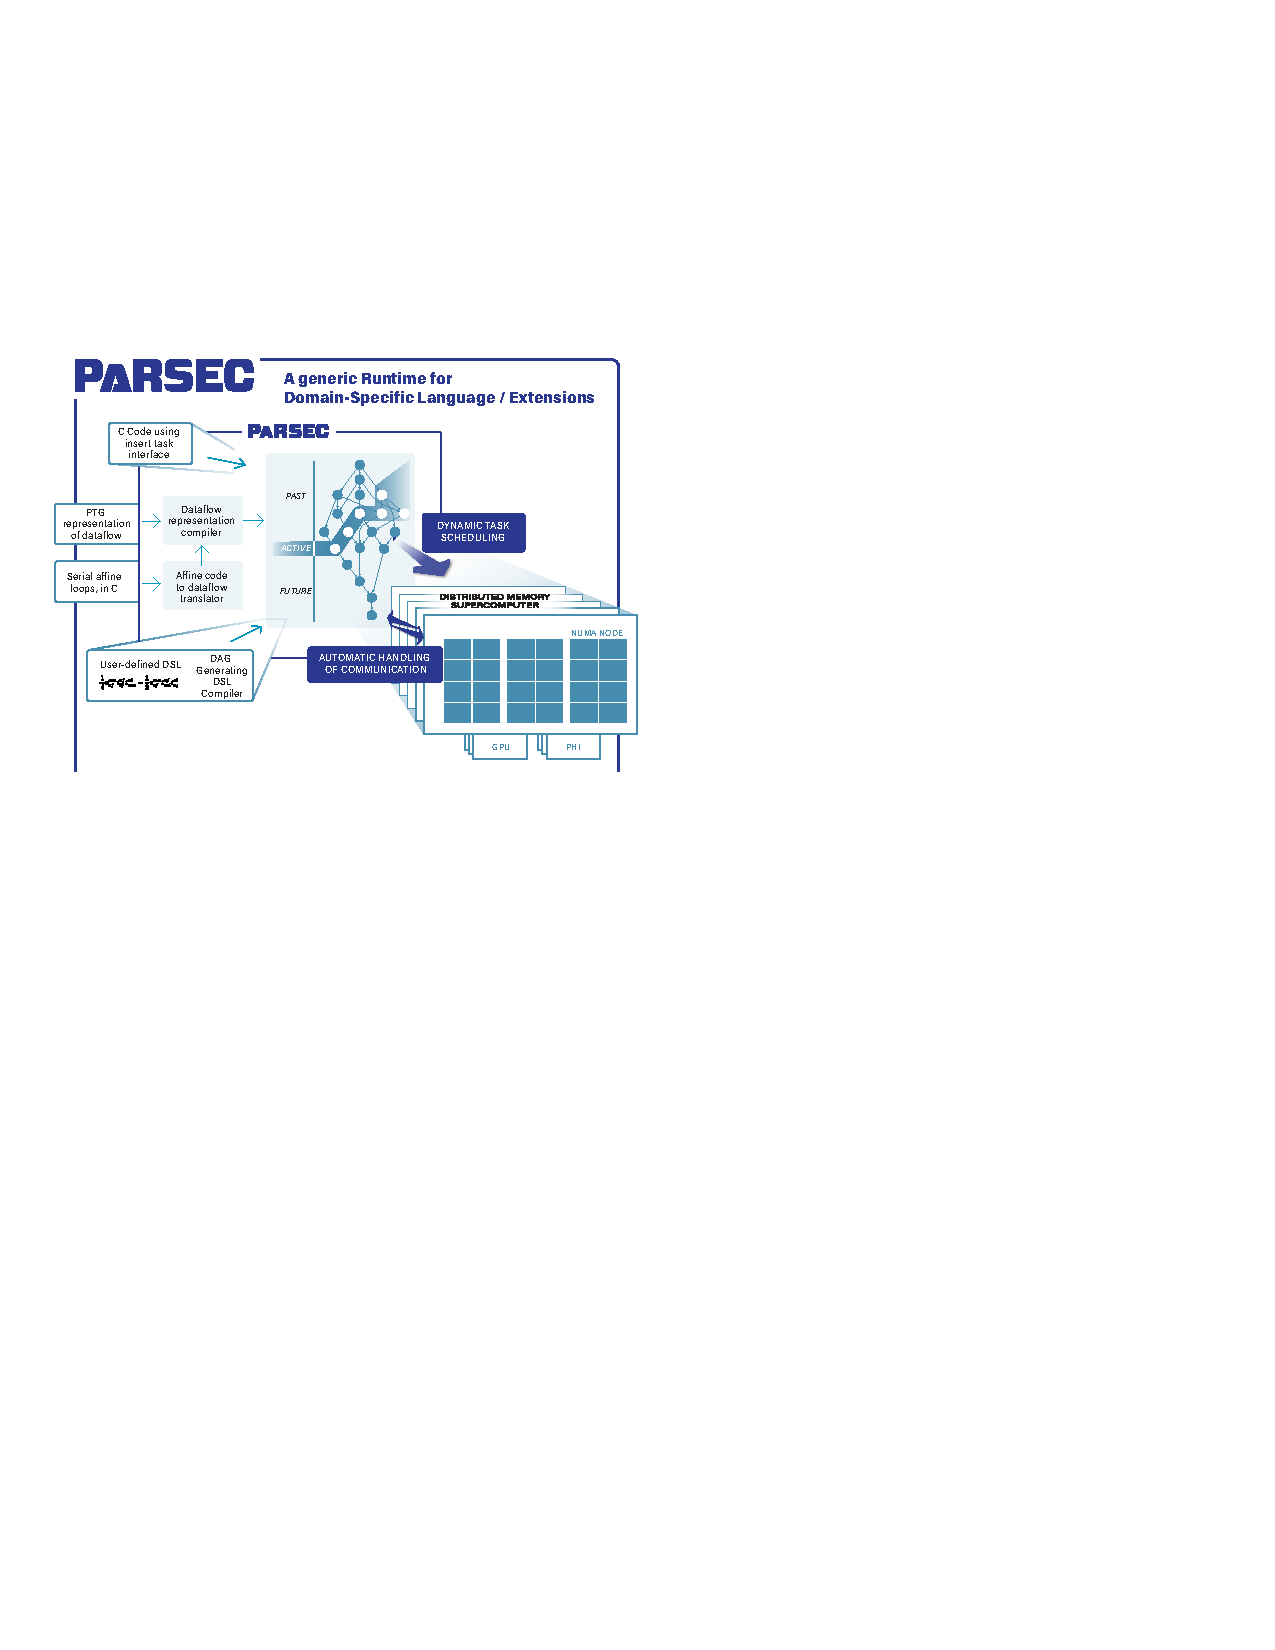
\includegraphics[width=.9\linewidth]{../parsec.pdf}
          
          \scriptsize PaRSEC: Parallel Runtime Scheduler and Execution Control
        \end{center}
        \begin{itemize}\scriptsize
        \item Task system for many micro tasks
        \item targets hybrid distributed large scale systems (e.g. Frontier)
        \item Available on all HPC systems via the Exascale Computing Project packages
        \end{itemize}
      \end{minipage}
    \end{column}\begin{column}{.7\linewidth}
      Support for task-based expression and execution in HPC
      \begin{itemize}
      \item How to manage asynchronous progress (of work, of communications)
      \item Promote separation of concerns: Algorithm expresses maximum parallelism, runtime maps to hardware
      \item Manage data hosting transparently (move data between nodes or devices in the background)
      \end{itemize}

      \bigskip

      \scriptsize PaRSEC software
      \begin{itemize}
      \item Provides various interfaces to program task systems (DSL, traditional 'insert-task' API, templated C++ interface for dynamic / computation-dependent DAGs)
      \item Comes with an ecosystem of tools (performance visualization, debugging)
      \end{itemize}
    \end{column}
  \end{columns}
  
\end{frame}

\begin{frame}
  \frametitle{My contributions related to PaRSEC}
  
  My major contributions related to \textcolor{brown}{PaRSEC}:
  \begin{itemize}
  \item Co-designer of the core engine
  \item Dynamic task schedulers, accelerator management
  \item Programming Interfaces 
    \begin{itemize}
    \item (Parameterized Task Graphs; Dynamic Task Discovery; Template Task Graphs)
    \end{itemize}
  \item Distributed Algorithms using or for PaRSEC
    \begin{itemize}
    \item Termination detection 
    \item Data redistribution
    \item Dense Linear Algebra
    \item Sparse Tensor Contraction -- \textcolor{red}{Application to Quantum Chemistry} 
    \end{itemize}
  \item Soft errors resilience in Task Systems
  \item Profiling and performance analysis ecosystem
  \end{itemize}
  
  PaRSEC software available by default on all HPC systems via the ECP packaging
  
  Significant impact on multiple communities (HiCMA -- \textcolor{red}{Gordon Bell finalist in 2022 with PaRSEC}; NWChemEX; MADNESS; MPQC; TiledArray; Chameleon; PASTiX)
    
\end{frame}

\section*{Resp.}

\begin{frame}
  \frametitle{Administrative and Pedagogical Responsibilities; Research Management}

  \begin{columns}
    \begin{column}{.45\linewidth}

      \scriptsize
      Research Management:
      \begin{myitemize}
        \myitem{PI of 2 NSF projects (\$2.5M), 1 ANR project}
        \myitem{CoPI of 1 STREP project}
        \myitem{CoPI of 3 NSF projects (\$2.7M)}
        \myitem{CoPI of 1 DoE project (\$4.7M)}
      \end{myitemize}

      \bigskip
      
      Advising (Master Interns, PhD students, software engineers and postdoc researchers):
      \begin{myitemize}
      \myitem{In France: 3 PhD students, 1 software engineer, 3 Master students}
      \myitem{In the USA: No official role of advisor in the USA, due to
        lack of tenure (policy of UTK). I worked closely with 7 PhD students, 3
        postdoctoral researchers, 8 master students (including some from
        ENS Lyon)}
      \end{myitemize}
  
%  thesards US: Qinglei Cao, Yu Pei, Reazul Hoque, Peng Du, Chongxiao Cao, Wesley Bland, Teng Ma
%  thesards FR: Camille Coti, Olivier Peres, Fatiha Bouabache
%  Ingenieur logiciel: Eric Rodriguez, 
%  postdoc: Joseph Schuchart, Amina Guermouche, Ala Rezmerita, Francois Lesueur, Damien Genet
%  Stagiaires M2 (ENS): Valentin Le Fevre, Julien Herrmann
%  Stagiaires M2 ou autre non ENS: Chunyan Tang, Hinde-Lilia Bouziane, Boris Collin, Michael Cadilhac, Vincent Bridonneau, Peter Gaultney

      \bigskip

      Pedagogical Responsibilities (as MdC in Paris-XI): year 1 to 3 of
      'ing\'enieurs par alternance' cursus for the informatics section -- class 2005, 2006, 2007
    \end{column}\begin{column}{.45\linewidth}\scriptsize
      Pedagogical Activities while at UTK:
      \begin{myitemize}
      \myitem{1 Research School -- 1 week $8\times 3h$}
      \myitem{13 Tutorials on Fault-Tolerance in HPC -- 1 day 8h}
      \myitem{4 Tutorials on task programming -- 1/2 day 4h}
      \end{myitemize}

      \bigskip

      Participation in committees:
      \begin{myitemize}
      \myitem{Executive Director for UTK in the JLESC since 2023}
      \myitem{Member of the directors committee of ICL at UTK, since 2014}
      \myitem{Member of the hiring committee (CSSU or CS) from Universit\'e
        Paris-XI from Sept 2006 to May 2010}
      \myitem{NSF Panelist in 2018, 2019}
      \end{myitemize}

      \bigskip

      Editorial responsibilities: Associate Editor of Journal of
      Parallel and Distributed Computing since 2022

    \end{column}
  \end{columns}
 
\end{frame}

\section{Research Program and Integration in ROMA}

\begin{frame}
  \frametitle{Task-based approaches $\Rightarrow$ sea-change in fault tolerance}

  \begin{center}
    \begin{tabular}{C{.4\linewidth}|C{.4\linewidth}}
      General-purpose FT & Application-specific FT \\\hline
      Coordinated checkpointing and rollback-recovery & Algorithm-Based Fault Tolerance  \\
      Replication                                     & Iterative convergence
    \end{tabular}

    \medskip
    
    \textcolor{blue}{HPC FT approaches have been designed for bulk-synchronous programming}
    
    \bigskip
  
    Task-based approach: asynchronous execution\\
    and dynamically scheduled independent tasks

    \bigskip
  
    \textcolor{red}{We need to redesign fault-tolerance in the context of task systems}
  \end{center}

\end{frame}

\frame{
  \frametitle{Opportunity and Challenge: Malleability}

  \begin{beamerboxesrounded}{Opportunity}
    \begin{center}
      \textcolor{red}{Task systems introduce generic malleability}
    \end{center}

    \begin{itemize}
    \item Tasks are units of work with identified inputs and outputs
    \item Runtime systems can migrate tasks to react to external condition changes (esp. process crash)
    \end{itemize}
  \end{beamerboxesrounded}

  Challenges:
  \begin{itemize}
  \item Non-linear performance degradation due to attrition
    \begin{itemize}
    \item[\frownie] Work and data placement is critical to algorithm performance and usually left to the programmer
    \item[\smiley] Crashed processes should be replaced, so performance degradation should only be transient
    \end{itemize}
  \item Redesign checkpointing as a per-task basis
    \begin{itemize}
    \item noncoordinated checkpointing and message logging
    \item selective replication
    \end{itemize}
  \end{itemize}
}

\frame{
  \frametitle{Applying ABFT to Task-Based Runtime Systems}

  \begin{itemize}
  \item ABFT: bulk-synchronous 'by nature'
    \begin{itemize}
    \item Need to keep the cheksum valid at each step
    \item Efficient \emph{because} checksum is updated by only extending synchronous operation
    \end{itemize}
  \item Task-Based Runtime Systems: asynchronous 'by nature'
    \begin{itemize}
    \item Add strict control flow to keep checksum up to date? \frownie
    \item How to react to failures? Conditional DAG?
    \end{itemize}
  \item ABFT + Tasks:
    \begin{itemize}
    \item Extend DAG with checksum / checksum update tasks
    \item Introduce scheduling priorities to make sure checksums are updated
    \item Define alternative paths to produce data, associate cost with paths
      \begin{itemize}
      \item A block can be computed by inversing the checksum
      \item but preferable path is to update directly
      \end{itemize}
    \end{itemize}
  \end{itemize}

  \begin{center}
    \textcolor{red}{Likely collaborations in NUMPEX}
  \end{center}
}

\begin{frame}
  \frametitle{Silent Data Corruption}

  SDCs are not well evaluated\footnote{In general we need more studies on faults in leadership systems and high-end systems}

  Intuition:
  \begin{itemize}
  \item They happen more often as the amount of memory grows
  \item They happen more often as the computational intensity grows
  \end{itemize}

  If the intuition is right, they will happen more and more frequently

  Application-specific fault tolerance can help
  \begin{itemize}
  \item Not necessarily (or not only) to correct failures
  \item But also to detect failures
  \end{itemize}

  \bigskip

  Challenge: Validation of computation is possible but \textcolor{red}{not reliable}

  \textcolor{red}{Ongoing work: how to (efficiently) use unreliable validation of work}

\end{frame}

\begin{frame}
  \frametitle{Fault tolerance as a tool for energy saving}

  \begin{itemize}
  \item Energy consumption of HPC centers becomes a problem (both economical and ecological)
    \begin{itemize}
    \item Current policy is to not bill allocation if a node within the allocation fails
    \item Some platforms are switching to bill-per-Joule
    \item Does it make sense to get 'free' Joules thanks to a node failure?
    \item Cloud-HPC convergence: CPUs are billed as soon as allocated, even if the application cannot be deployed
    \end{itemize}
  \item Using stranded energy in Cloud or HPC
    \begin{itemize}
    \item Non-dispatchable renewable energy sources to power HPC
    \item $\Rightarrow$ Power cost varies with time (soft version)
    \item $\Rightarrow$ Power capping varies with time (hard version)
    \item $\Rightarrow$ Job scheduler may have to kill apps. Resilience can help.
    \end{itemize}
  \end{itemize}
  \begin{center}
    \textcolor{red}{Fits well the Energy Minimization topic in ROMA}
  \end{center}
\end{frame}



\section{Projet d'Enseignement}

%% \begin{frame}
%%   \frametitle{Syst\`eme d'Exploitation}
  
%%   \begin{beamerboxesrounded}{But du cours}
%%     \begin{itemize}
%%     \item Vue d'ensemble du fonctionnement des syst\`emes d'exploitation
%%     \item Composants physiques d'un ordinateur, interactions, interface
%%     \item Repr\'esentation abstraite de la machine
%%     \item Compr\'ehension des co\^uts (m\'emoire ou temps) li\'es aux diff\'erentes op\'erations 
%%     \end{itemize}
%%   \end{beamerboxesrounded}
  
%%   \bigskip
  
%%   \small R\'ef\'erences:\\
%%   $[1]$ Silberschatz, Abraham, and Peter Baer Galvin. "Operatings System Concepts." (2013).\\
%%   $[2]$ Tanenbaum, Andrew. Modern operating systems. Pearson Education, Inc., 2009.\\
%%   $[3]$ Arpaci-Dusseau, Remzi H., and Andrea C. Arpaci-Dusseau. Operating systems: Three easy pieces. Arpaci-Dusseau Books, LLC, 2018.
  
%% \end{frame}

%% \begin{frame}
%%   \frametitle{D\'ecoupage du cours (Syst\`emes d'Exploitation)}

%%   \begin{columns}
%%     \begin{column}{.45\linewidth}
%%       \begin{description}
%%       \item[Introduction] {\footnotesize Histoire des OS, r\^oles, conceptions}
%%       \item[Processus] {\footnotesize Concept de processus, partage de temps, ordonnancement, communication inter-processus}
%%       \item[Synchronisation] {\footnotesize Gestion des interd\'ependances, exclusion mutuelle, s\'emaphores, priorit\'es}
%%       \item[M\'emoire] {\footnotesize M\'emoire virtuelle, pagination, politiques d'\'eviction, support mat\'eriel}
%%       \end{description}
%%     \end{column}\begin{column}{.45\linewidth}
%%       \begin{description}
%%       \item[Stockage] {\footnotesize Gestion des entr\'ees-sorties, interfaces, structures et fonctions internes}
%%       \item[Syst\`eme de fichiers] {\footnotesize Hi\'erarchie, r\'epertoire, volumes; journalisation, aggr\'egation et fiabilisation des ressources}
%%       \item[S\'ecurit\'e] {\footnotesize Droits d'acc\`es (fichiers, CPU, m\'emoire), isolation, contr\^ole d'acc\`es, redondance}
%%       \end{description}
%%     \end{column}
%%   \end{columns}

%%   \smallskip
  
%%   Sujets additionels: R\'eseaux et syst\`emes distribu\'es (TCP/IP); virtualisation
%% \end{frame}

\begin{frame}
  \frametitle{Syst\`emes Distribu\'es}
  
  \begin{beamerboxesrounded}{But du cours}
    \begin{itemize}
    \item Introduction aux syst\`emes distribu\'es
    \item Modes de communication (passage de message et m\'emoire partag\'ee)
    \item Probl\`emes fondamentaux (exclusion mutuelle, synchronisation, topologies couvrantes, routage, distribution de donn\'ees, \ldots)
    \item Tol\'erance aux fautes (d\'et\'ecteurs de fautes, \'election de leader, crash, erreurs transitoires, processus byzantins)
    \end{itemize}
  \end{beamerboxesrounded}
  
  \bigskip
  
  \small R\'ef\'erences:\\
  $[1]$ Taubenfeld, Gadi, Distributed Computing Pearls. Morgan \& Claypool, 2018\\
  $[2]$ Raynal, Michel, Distributed Algorithms for Message-Passing Systems. Springer, 2013\\
  $[3]$ Tel, Gerard, Introduction to Distributed Algorithms (2nd Edition). Cambridge University Press, 2000
  
\end{frame}

\begin{frame}
  \frametitle{Projet Int\'egr\'e}

  \begin{columns}
    \begin{column}{.45\linewidth}\small
      Buts:
      \begin{itemize}
      \item Acqu\'erir de l'exp\'erience en programmation imp\'erative (C, Python, C++, ...)
      \item Apprendre le g\'enie logiciel par la pratique (d\'efinition d'un cahier des charges, d'une interface, des m\'ethodes de test; avoir une conception modulaire d'un projet cons\'equent)
      \item Apprendre \`a travailler de mani\`ere collaborative (ma\^\i{}trise des outils logiciels -- git, gitlab, etc... -- mais aussi apprendre \`a travailler en groupe)
      \end{itemize}
    \end{column}\begin{column}{.45\linewidth}\small
      Mon exp\'erience dans le domaine:
      \begin{itemize}
      \item suivi de projets (TER) en tant que MdC
      \item dans le cadre de ma recherche : participation \`a plusieurs projets logiciels open source d\'evelop\'es en communaut\'es (PaRSEC 82,973 LOC, 20+ contributeurs; dplasma 90,844 LOC, 10+ contributeurs; TTG, 37,500 LOC, 6+ contributeurs; ULFM in Open MPI, 236,570 LOC, 50+ contributeurs)
      \end{itemize}
    \end{column}
  \end{columns}
\end{frame}

\begin{frame}
  \frametitle{Programmation Parall\'ele: enjeux, outils, et recherche}

  \begin{beamerboxesrounded}{But du cours}
    Introduction \`a la programmation parall\'ele pour le calcul \`a haute performance (HPC). \'Etat de l'art des environnements mat\'eriel et logiciel, et introduction des probl\'ematiques de recherche l\'iees au HPC.
  \end{beamerboxesrounded}

  \bigskip
  
  \small R\'ef\'erences:\\
  $[1]$ Hager, Georg, and Gerhard Wellein. Introduction to high performance computing for scientists and engineers. CRC Press, 2010.\\
  $[2]$ Sterling, Thomas, Maciej Brodowicz, and Matthew Anderson. High performance computing: modern systems and practices. Morgan Kaufmann, 2017.\\
  $[3]$ Dongarra, Jack, Thomas Herault, and Yves Robert. Fault tolerance techniques for high-performance computing. Springer International Publishing, 2015.
  
\end{frame}

\begin{frame}
  \frametitle{Ce que je peux amener au d\'epartement}

  \begin{columns}
    \begin{column}{.55\linewidth}
      Cours de la maquette existante sur lesquels je peux intervenir imm\'ediatement:
      \begin{itemize}\small
      \item Architecture des ordinateurs et syst\`eme d'exploitation (L3/1\`ere ann\'ee)
      \item R\'eseaux (L3/1\`ere ann\'ee)
      \item Programmation (L3/1\`ere ann\'ee)
      \item Projet Int\'egr\'e 1/2 (M1/2\`eme ann\'ee)
      \item Algorithmique et Programmation Parall\`ele et Distribu\'ee (M1/2\`eme ann\'ee)
      \item Syst\`emes Distribu\'es (M1/2\`eme ann\'ee)
      \item \'Evaluation de Performances (M1/2\`eme ann\'ee)
      \end{itemize}
    \end{column}\begin{column}{.4\linewidth}
      \small
      Ma recherche : \\
      Mod\'elisation et \'evaluation exp\'erimentale d'algorithmes parall\`eles et distribu\'es pour le HPC

      \bigskip
      
      Je peux faire d\'ecouvrir aux \'etudiants de l'ENS l'approche exp\'erimentale, et la mise en pratique des th\'eories enseign\'ees, dans un contexte de recherche, et les inciter \`a poursuivre en th\`ese sur ces aspects.

      \bigskip

      Je suis pr\^et \`a m'investir dans les charges administratives li\'ees au d\'epartement.
      
    \end{column}
  \end{columns}
  
\end{frame}

\section{Conclusion}

\begin{frame}
  \frametitle{Pourquoi je souhaite \^etre professeur \`a l'ENS de Lyon}

  Recherche:
  \begin{itemize}
  \item Un environnement id\'eal pour d\'eveloper mes th\`emes de recherche
  \item Renforcer les collaborations et \'echanges avec les membres de l'\'Equipe ROMA, du LIP, et la communaut\'e Fran\c{c}aise du HPC et du syst\`eme
  \item Cr\'eer des ponts entre th\'eorie et pratique
  \item Attirer de jeunes chercheurs brillants sur la tol\'erance aux fautes et les syst\`emes de t\^aches dans le HPC
  \end{itemize}

  Enseignement:
  \begin{itemize}
  \item Retourner \`a l'enseignement apr\`es la pause forc\'ee durant mon s\'ejour aux \'Etats-Unis
  \item Cr\'eer des ponts entre th\'eorie et pratique
  \item Apporter une culture de l'informatique en tant que science exp\'erimentale
  \item \'Etendre le spectre des domaines dans lesquels les \'etudiants de l'ENS peuvent d\'eveloper une carri\`ere
  \end{itemize}
  
\end{frame}


\end{document}
